\documentclass[conference]{IEEEtran}
\IEEEoverridecommandlockouts
% The preceding line is only needed to identify funding in the first footnote. If that is unneeded, please comment it out.
\usepackage{cite}
\usepackage{amsmath,amssymb,amsfonts}
\usepackage[fleqn]{mathtools}
\usepackage{algorithmic}
\usepackage{graphicx}
\usepackage{textcomp}
\usepackage{xcolor}
\usepackage{array}
\usepackage{multirow}
\def\BibTeX{{\rm B\kern-.05em{\sc i\kern-.025em b}\kern-.08em
    T\kern-.1667em\lower.7ex\hbox{E}\kern-.125emX}}

\usepackage{fancyhdr}
\usepackage{lastpage}

\pagestyle{fancy}
\fancyhf{}

\rfoot{Page \thepage \hspace{1pt} of \pageref{LastPage}}

\begin{document}

\title{Human Presence and Activity Detection from WiFi CSI Data using CNN\\
% \thanks{Identify applicable funding agency here. If none, delete this.}
}

\author{\IEEEauthorblockN{Md Touhiduzzaman}
\IEEEauthorblockA{\textit{Department of Computer Science} \\
\textit{Virginia Commonwealth University}\\
Richmond, Virginia, USA \\
touhiduzzamm@vcu.edu}
\and
\IEEEauthorblockN{Maher Al Islam}
\IEEEauthorblockA{\textit{Dept. of Electrical \& Computer Engineering} \\
\textit{Virginia Commonwealth University}\\
Richmond, Virginia, USA \\
alislamm@vcu.edu}
\and
\IEEEauthorblockN{Samah Ahmed}
\IEEEauthorblockA{\textit{Department of Computer Science} \\
\textit{Virginia Commonwealth University}\\
Richmond, Virginia, USA \\
ahmedss5@vcu.edu}
}

\maketitle

\begin{abstract}
WiFi sensing can be used to monitor specific human movements and also to predict the movements after learning it using any machine learning paradigm. In this project, a convolutional neural network is implemented for a large dataset of human mobility through a WiFi network delivering CSI data with so many variations. The hyperparameter optimization technique is used to find out specific values of several parameters of the machine learning model to predict 12 different human activities with $73.3\%$ of accuracy at the best case. While there are other HAR models performing better than our accuracy, the novelty of the paper lies in applying the convolutional neural-network (CNN) to predict from a larger number of human actions performed by 9 different persons of varying features and in 3 different environment setups. Considering $69.78\%$ as the best accuracy of other studies with similar degree of variations and actions, our approach can be considered slightly better and obviously novel in using CNN in this field.
\end{abstract}

\begin{IEEEkeywords}
CNN, WiFi, sensing, CSI, machine learning, human activity detection, surveillance
\end{IEEEkeywords}

\section{Introduction}
% Why WiFi Sensing
In this era of conflict between surveillance and privacy concerns, WiFi sensing brings a very optimal lineup to monitor necessary surveillance data pruning through unnecessary personal details by the implementation. It also benefits through lower data storage and processing time than camera recorded video or image data. Therefore, to implement any surveillance system where specific movements are needed, one need not record heavy cam-feeds and occupy huge processing overhead, rather can use WiFi channel state information (CSI) data to learn the specification of the movements and then classify those.

% Why CNN
Channel State Information (CSI) obtained from commercial WiFi chipsets has proven to be efficient in detecting human interactions inside any radio wave. Due to high availability \& practical usability, the WiFi network can be the most effective radio network to collect CSI data. The popularity of approaches that measure Received Signal Strength (RSS) by narrowband radio devices is due to cost-effectiveness and ubiquity. However, recent progress in signal descriptors, such as CSI, obtained through low-cost chipsets like ESP32, Intel 5300 NIC, and IEEE 802.11n chipsets offer enhanced accuracy compared to RSS. Due to high temporal variance in RSS, slow movements of humans end up hidden in the inherent signal variability \cite{a1}. Comparatively, the structure of CSI is temporally more stable than RSS because it captures small-scale multipath propagation over multiple sub-carriers in frequency domain \cite{a2} \cite{a3}. CSI indicates different physical qualities of the channel, such as shadowing, frequency selective fading, multipath propagation, and interference effects. Hence, CSI is currently a good alternative for RSS.\\
Compared to traditional technologies, CSI-based detection has several advantages. It detects humans through walls, does not depend on lighting, preserves user privacy, and importantly, occupants are not required to carry any devices. Hence, it is widely used to quantify the human presence interaction with the wireless channel in the form of occupancy detection, activity/gesture/identity recognition, and human positioning.\\

The attributes of WiFi CSI data vary depending on routers and network specifications. The values are also hugely impacted by the orientation of the environment, i.e., the room structure, furniture in the room, openings as doors or windows in the room, moving items like flying curtains, ambient or any other sound,  etc. These variations are difficult to characterize by naked human realization. That is why a blind machine learning paradigm like a deep neural network, convolutional neural network, and so on can be used to train and classify the CSI dataset. In this project, a convolutional neural network (CNN) with 2 hidden layers in conjunction with 1 reshape layer and 2 dense-layers is implemented. The neural network trains a weight array by the larger portion of the dataset and then implies the weight array directly over the test dataset, which is a subset of the whole collection of the CSI dataset.

\begin{figure}[htbp]
\centerline{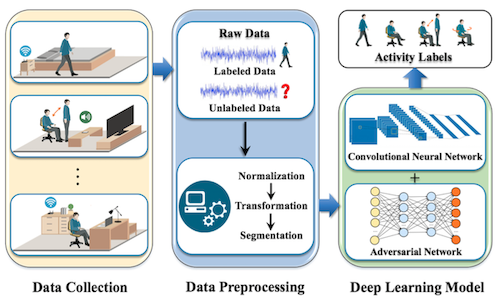
\includegraphics{images/system_framework.png}}
\caption{System Framework}
\label{fig_sys_framework}
\end{figure}

\begin{figure*}[htbp]
\centerline{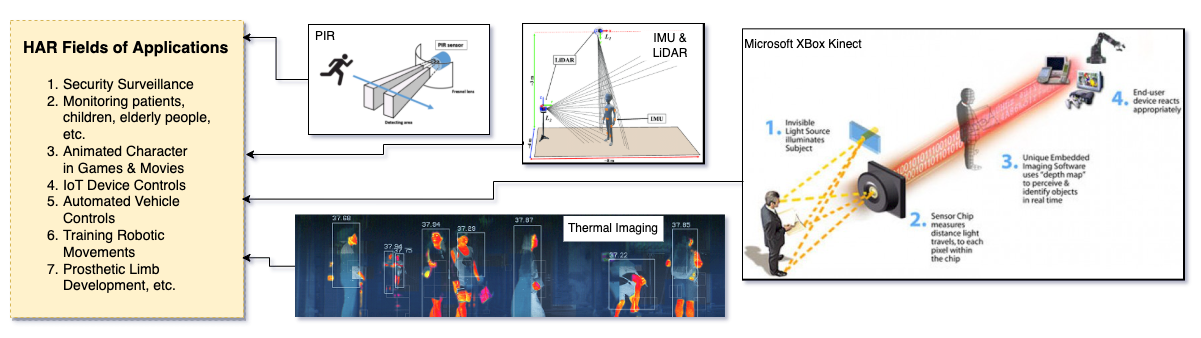
\includegraphics[scale=0.45]{images/har_categories.png}}
\caption{Different Applications of HAR using Several Sensors (Image Credits \cite{img_har_categories} \cite{imu_lidar})}
\label{fig_har_categories}
\end{figure*}

\section{Background \& Related Works}
Human Activity Recognition (HAR) has been a very much explored research arena. These researches have been spanned from surveillance \& monitoring to animated movie and gaming, controlling Internet of Things (IoT) devices through various gestures, automated vehicle controls, robotic evolution, etc. Most of the researches have been done using camera feeds, smart wearable devices and using several other sensors like - infrared (IR), passive infrared (PIR), Microsoft XBOX Kinect, IMU (Inertial Measurement Unit) \cite{imu_human}, thermal imaging, ultrasound, pyroelectric infrared \cite{pyroelectric_human1}, \cite{pyroelectric_human2}, etc.
However, there are only a few researches done using WiFi sensed CSI data. All of these researches can be discussed in three sections -
\begin{enumerate}
\item Various methods of HAR,
\item HAR using WiFi sensing CSI data and
\item Novelty of our work
\end{enumerate}
\subsection[iia]{Various Methods of Human Activity Recognition}
\label{har_sensors}
Various custom sensors are experimented to detect several human activities in many studies and several are already in the public market, like Microsoft XBOX Kinect, IMU, PIR, Rokoko smartwears \cite{rokoko_link}, etc.\\
Even for a very subtle movements like fingers \& wrists, we can refer some quite ingenious studies using custom made sensors. In \cite{mmWave_rf_vs_kinect_radar_img}, a mmWave based radio frequency is shown to be analyzable and so learnable using CNN that rehab movements of any injured one of the 19 joints in human hand can be monitored using the custom made wireless sensor. An comparison with radar imaging is also shown in that study, where their implementation is claimed to be performing better than that in this specific case of hand rehab. This sensor is also claimed to be consuming least amount of energy ($443\mu J$) and least amount of time ($64\mu s$) than any sensors present in the market.\\
In another similar study \cite{math_dervd_hand_pos_sensor}, a sensor is designed using mathematical derivation for least Root Mean Square Error (RMSE) to detect one wide-arm exercise of any human. The advantage of the sensor is claimed to be of miniature in size and very much portable. In another study \cite{wear_handglove}, a wearable soft smargloves is designed as a sensory \& motor glove. It can classify 16 separate finger gestures used in mirror therapy \& task-oriented therapy with upto 93.32\% accuracy using SVM, kNN \& DT algorithms.\\
Another study uses Multi-Dimensional Dynamic Time Warping (MDTW) model using MatLAB model and Leap Motion (LM)\cite{ultraleap} sensors to detect four hand gestures using a robotic hand simulation. Another study \cite{joints_imu} uses IMU sensors to classify several movements of shoulder, hip, knee and elbow. Dynamic Time Warping (DTW) is used in this study.\\
Moving towards bigger movement detection, we can refer to Dalal et. al. \cite{dalal}, where any human movement in a motion capture video recording is shown to be detectable for even examples having more than 4400 human. Yin et. al. \cite{yun_pir} uses only 2 pairs of Pyroelectric Infrared sensors to classify the speed, distance and direction any human movement with 94\% accuracy. In another research by Park et. al. \cite{young_impulse_radar}, it is shown by experiments that impulse radar signals can be used to detect human presence and motion with almost 100\% accuracy.
Jeong et. al.\cite{jeong_thermal} developed a probabilistic method to detect human subjects using even a low-resolution thermal imaging sensor. It covers various pre and post-image processing methods including background collection, Gaussian filtering, segmentation, local/global adaptive threshold and background learning. Patil et. al. \cite{imu_lidar} uses a combination of multiple LiDAR sensors Inertial Motion Unit (IMU) sensors to identify various poses for a human in motion, even at real time. States of the different moving joints of human limbs for different walking style are classified using multiple IMU sensors in another study by Semwal et. al. \cite{semwal}.
In general, these used sensors have been very costly or designed using a complex process that may be difficult to maintain as per the course of usage. All of these studies can be countered by our proposal with only one statement that - our proposed WiFi sensing setup can be extended to function without any kind of extra hardware setup, but only by using the traditional WiFi routers, which can be easily found around us now a days. Therefore, our proposed system may outperform these studies in the matter of practical usability.

\subsection{Human Activity Recognition using WiFi Sensing}
\label{har_wifi}
There have been comparatively very few studies using WiFi sensing as a medium of detecting human activities and gestures. Wu \& Zhang et. al. proposes DeMan\cite{deman} system, which is a unified scheme for non-invasive detection of moving and stationary human on commodity WiFi devices. Extensive experimental evaluation in typical indoor environments validates the performance of DeMan in various human poses and locations and diverse channel conditions. Particularly, DeMan provides a detection rate of around 95\% for both moving and stationary people, while identifies human-free scenarios by 96\%. But this study skips any specific action of a moving human being inside their proposed network.\\
Domenico et. al. \cite{domenico} proposes a WiFi-based through-the-wall (TTW) presence detection of stationary and moving humans by analyzing the doppler spectrum. However, their proposal includes two WiFi routers on each side of the wall, which may be impractical in many scenarios. Another study by Hernandez et. al. \cite{hernandez_one_sided_wall} proposes a one-sided wall occupancy monitoring, where it is shown that a single WiFi signal receiver device is enough to sense any human walking even on the opposite side of any wall and keep a count of them. In another study by Hernandez et. al. \cite{hernandez_wifederate}, a system called WiFedarate is proposed, which implements an edge based federated learning over WiFi sensing. The proposed WiFederated system can scale as more locations and scenarios for learning are added and it provides a more accurate and time efficient solution compared to existing transfer learning and adversarial learning solutions using the parallel training ability at multiple clients. By introducing new client selection methods during the federated-learning process, the accuracy is shown to increase further and then the feasibility of training models at the edge and introduce continuous annotation to allow for continuous learning over time is evaluated to be good.\\
WiFi network's CSI data is explored in a study by Palipana et. al. \cite{csi_human}. Using CSI data, they have modeled the human presence and then analysed the occurrences of non-linear correlations among the WiFi sub-carriers. Then they have exploited these correlations by introducing non-linear techniques to reduce CSI dimensions and filter noise, which can detect human presence and movements even when human motion is insignificant or occurs very far from the link. Their non-linear techniques improve the detection accuracy up to 5\% compared to the linear approach with just two transceivers.\\
A very interesting study by Liu et. al. \cite{liu_breathing} proposes a CSI analyzing technique which can detect static human through estimating the breathing frequency by exploring phase information of CSI. They achieved more robust data by fusing subcarriers and filtered out environmental noise by adopting Butterworth filter and using hampel filter before and during wavelet denoising. For estimating the frequency, they introduced Fast Fourier Transformation (FFT), Estimating Signal Parameter via Rotational Invariance Techniques (ESPRIT) and Multiple Signal Classification (MUSIC). The results of their study show that human detection accuracy can achieve higher than 95\% and averaged evaluating accuracy can reach 89.8\% with their system.\\
However, none of these studies have covered the detection of human presence and movements in a specific room with any neural network based learning.

\subsection{Novelty of Our Work}
%other sensors - power, cost, setup complexity, maintenance cost, processing cost\\
As we have already have discussed in \ref{har_sensors}, the proposed sensors are either costly, consume extra power, complex to design and maintain, costly to maintain or costly to process the information. So, those custom sensory developments can be trumped over by our approach with more commonly available and maintainable WiFi networks.\\
%other WiFi sensing - not DNN, impact of various activation functions, faster processing
Moreover, none of the human detection systems using WiFi sensing, as discussed in \ref{har_wifi}, considers both stationary and moving human at the same time and processes it with more complex signal processing algorithms. Our proposal excludes any complex preprocessing of the raw CSI data, other than calculating the plain amplitude of the signals from those data, and then runs a deep neural network model over them to detect any human presence and movement. From this point of view, our work is novel and different from any other existing approaches to detect human motion.




\section{Problem Statement}
\label{section_problem_statement}
There are various implementations of human activity recognition. However, the purpose of this problem is to identify as many common human actions as can be detected, like - entering into a room, walking around the room, standing or sitting idle in the room, exiting the room, etc.
In other words, we can state the problem as - if a person $S$ does any action $a_i$, such that $a_i \in A=\{a_1, a_2, a_3, ..., a_n\}$ within a specific environment ${E}$, the problem requires us to classify that action within a predefined set of classes $C=\{c_1, c_2, c_3, ..., c_n\}$.



\section{Solution Proposal}
We have divided the problem stated in \ref{section_problem_statement} into three sub-problems as shown in Figure \ref{fig_sys_framework}, like -
\begin{enumerate}
\item Data Collection
\item Data Preprocessing
\item Deep Learning Model
\end{enumerate}
Our solution apporaches for all of these subproblems are described in the following subsections.

\subsection{Data Collection}
We have used the dataset provided in Alsaify et. al \cite{dataset}. In this dataset, thirty people have been studied in three environments, in both LOS and NLOS setups. However, we have used 10 out of 30 people for our experiment. The average age, height, and weight of the participants were 22.7 2.95 years, 178.37 8.4 cm, and 81.9 18.16 kg, respectively. The data collected for ten distinct subjects is available in each sub-directories as shown in TABLE I. Each individual completed five experiments, each of which was repeated 20 times. There are a total of 300 files in the sub-directory linked with each environment. A Multi-Input Multi-Output (MIMO) system was employed with these configurations, consisting of 13 Wi-Fi streams. For each stream, the CSI tool used to capture Wi-Fi signals at the receiving NIC can capture up to 30 CSI subcarriers. To put it another way, the dataset captures 3*30 CSI subcarriers.




\begin{table}
    \begin{tabular}{| c|c|c |} 
     \hline
     Symbol	& Abbreviation For & Range\\ [0.2ex]
     \hline
     E	& Environment &	\multicolumn{1}{|l|}{$$\{1, 2, 3\}$$}\\ [1ex] 
     S	& Subject	& \multicolumn{1}{|l|}{$$\{1, 2, 3, 11, 12, 13, 21, 22, 23\}$$}\\ [1ex] 
     C	& Experiment Class	& \multicolumn{1}{|l|}{$$\{1, 2, 3, 4, 5\}$$}\\ [1ex] 
     A	& Activity	& \multicolumn{1}{|l|}{$$\{1, 2, 3, ..., 12\}$$}\\ [1ex] 
     T	& Trial	& \multicolumn{1}{|l|}{$$\{1, 2, 3, ..., 20\}$$}\\ [1ex]
     \hline\hline
    \end{tabular}
\caption{\label{tab:table_naming} naming conventions in the dataset}
\end{table}

\begin{table}
\begin{center}
    \begin{tabular}{| m{0.5cm} | m{1.5cm}| m{0.75cm} | m{4cm} |}
    
    \hline
    Expt. ID & Expt. & Activity & Description\\ [1ex]
    \hline\hline
    \multirow{3}{3em}{C1}	& \multirow{3}{3em}{Falling from sitting}  & A1	& Sit still on a chair\\ [1ex]
        &                                & A2	& Falling down\\ [1ex]
        &                                & A3	& Lie down\\ [1ex]
    \hline
    \multirow{3}{2em}{C2}	& \multirow{3}{2em}{Falling from standing} & A4	& Stand still\\ [1ex]
        &                                & A5	& Falling down\\ [1ex]
        &                                & A3	& Lie down\\ [1ex]
    \hline
    \multirow{4}{4em}{C3}	& \multirow{3}{3em}{Walking}                & A6	& Walking from transmitter to receiver\\ [1ex]
        &                                & A7	& Turning\\ [1ex]
        &                                & A8	& Walking from receiver to transmitter\\ [1ex]
        &                                & A9	& Turning\\ [1ex]
    \hline
    \multirow{4}{4em}{C4}	& \multirow{3}{3em}{Sit down \& stand up}   & A1	& Sit still on a chair\\ [1ex]
        &                                & A10	& Standing up\\ [1ex]
        &                                & A4	& Stand still\\ [1ex]
        &                                & A11	& Sitting down\\ [1ex]
    \hline
                    C5	    & Pick pen	 & A12	& Pick a pen from the ground\\ [1ex]
    \hline\hline
    \end{tabular}
\end{center}
\caption{\label{tab:table_actions} Fields contained within the structure of the captured Wi-Fi packets}
\end{table}

\begin{table}
    \begin{tabular}{|| c | c | c | c | c | c | c||} 
     \hline
     Env. & Config. & Subject\newline ID & Age \newline (years) & Weight\newline (kg) & Height\newline (cm)\\ [0.2ex]
     \hline\hline
     1	& LOS	& S1	& 35    & 75	& 176\\ [1ex] 
        &       & S2	& 21    & 63	& 188\\ [1ex] 
        &       & S3	& 25    & 75	& 184\\ [1ex] 
     \hline
    2	& LOS	& S11	& 23	& 93	& 180\\ [1ex] 
        &       & S12	& 26	& 60	& 178\\ [1ex] 
        &       & S13	& 20	& 98	& 188\\ [1ex] 
     \hline
    3	& NLOS  & S21	& 21	& 70	& 180\\ [1ex] 
        &       & S22	& 22	& 94	& 186\\ [1ex] 
        &       & S23	& 21	& 91	& 192\\ [1ex] 
     \hline\hline
    \end{tabular}
\caption{\label{tabtable_subjects}Environments' details along with the subject's info}
\end{table}
  
The dataset \cite{dataset} contains three different environment setup as shown in Figure\ref{fig_room_schematics}. In the first environment, the Wi-Fi signals were captured in their research laboratory. The dimensions of the laboratory are 4.7 m ×4.7 m. The transmitter and the receiver were placed at 3.7 m apart from each other. Fig. 3 a shows a sketch of the environment, while Fig. 3 b shows an image of the environment. All subjects were instructed to perform the pre-explained activities in the middle location between the transmitter and the receiver. In the second environment, the Wi-Fi signals were captured in a university hallway of dimensions 7.95 m ×3.6 m. In this environment, the transmitter and the receiver were placed at 7.6 m apart from each other. Fig. \ref{fig_room_schematics}a shows a sketch of this environment while Fig. 3b shows an actual image of the environment. As before, the subjects were instructed to perform their pre-explained activities near the centre between the transmitter and the receiver.

The experiments performed in the third environment differ from the experiments carried out in the first and the second environments in the sense that there was a barrier between the subject performing the experiment and the device capturing the Wi-Fi signals. In other words, the transmitter and the receiver were in a NLOS configuration. Specifically, in the third environment, there was a barrier wooden wall with thickness of 8 cm between the transmitter and the receiver. The transmitter was placed outside the room while the receiver was placed inside the room. The distance between the transmitter and receiver was fixed at 5.44 m. An illustration and an image of the third environment is provided in Fig. \ref{fig_room_schematics}c.

An excerpt of the collected CSI data is given in the table \ref{table:csi_raw}, where $timestamp\_low$ indicates a reading from internal clock ticks of the Intel 5300 NIC and $rate$ indicates the frequency (in Hz) at which WiFi signals are transmitted and received. This table shows the collected raw CSI in complex number format as $x+iy$, as collected directly from the NIC. Each CSI column is named as $csi\_e\_a\_s$, where $e$ is the environment number, $a$ is the  antenna number and $s$ is the subcarrier number.\\
The table \ref{table:csi_processed} lists down the processed CSI data with respective activity labels in range of $\{1, 2, 3, ..., 12\}$. Each CSI value is converted to its corresponding amplitude form from its complex number ($x+iy$) format, using the formula: $A = \sqrt{x^2 + y^2}$.


\begin{table}
    \begin{tabular}{| c | c |c | c | c| c|} 
     \hline
     timestamp\_low & rate & csi\_1\_1\_1 & csi\_1\_1\_2 & ... & csi\_1\_3\_30\\ [0.2ex]
     \hline\hline
     86147562 & 256 & 15+15i & 23+-7i & ... & -6+16i \\ [1ex]
     \hline
     86150687 & 256 & -19+3i & -9+22i & ... & 10+-12i \\ [1ex]
     \hline
     86153800 & 256 &  2+22i &  23+9i & ... & -14+12i \\ [1ex]
     \hline
     ... & ... &  ... &  ... & ... & ... \\ [1ex]
     \hline
     89147467 & 256 & -11+15i & 6+22i & ... & -16+-7i \\ [1ex]
     \hline\hline
    \end{tabular}
\caption{\label{table:csi_raw}Sample of a few raw CSI data Collected from Intel 5300 NIC}
\end{table}

\begin{table}
    \begin{tabular}{| c | c |c | c | c| c|} 
     \hline
     timestamp\_low & Label & csi\_1\_1\_1 & csi\_1\_1\_2 & ... & csi\_1\_3\_30\\ [0.2ex]
     \hline\hline
     86147562 & 1  & 21.21 & 24.04 & ... & 17.09 \\ [1ex]
     \hline
     86150687 & 1  & 19.24 & 23.7  & ... & 15.62 \\ [1ex]
     \hline
     86153800 & 1  & 22.09 & 24.70 & ... & 18.44 \\ [1ex]
     \hline
     ... & ... &  ... &  ... & ... & ... \\ [1ex]
     \hline
     89147467 & 12 & 25.94 & 26.93 & ... & 21.84 \\ [1ex]
     \hline\hline
    \end{tabular}
\caption{\label{table:csi_processed}Processed \& activity-labeled CSI from the complete dataset}
\end{table}


In our specific implementation, we have concentrated on implementing an efficient deep learning model, i.e., the third sub-problem, while a pre-processed proven dataset is used from an open-source collection \cite{dataset}. During the dataset collection process as shown in \cite{dataset}, ten activities are done in four specific room setups by two different people.
Therefore, referring to section \ref{section_problem_statement}, we can specify our problem variables as -
\begin{enumerate}
\item Set of environments, $E = \{e_1, e_2, e_3\}$,
\item Set of classes, $C = \{c_1, c_2, c_3, c_4, c_5 \}$,
\item Actions, $A = \{a_1, a_2, a_3, ..., a_{11}, a_{12}\}$,
\item Set of persons, $S = \{s_1, s_2, ..., s_{32}, s_{33}\}$
\end{enumerate}


The dateset are collected in three different environments. For the first and second environments, we captured Wi-Fi signals in the LOS configuration. For the third environment, the NLOS configuration was used.

The schematics of the three rooms are shown in Figure \ref{fig_room_schematics}.  Inside each of those rooms, an Intel 5300 NIC Device \cite{intel_nic_device} acts as the access-point (AP), while three Raspberry Pi clients connect with the AP. CSI \& RSS data are collected for each of those three client-AP connection pairs. We have not used RSS data as it is shown CSI dataset is enough to classify actions rather than complicating things using RSS \cite{a1} \cite{a2} \cite{a3}. The CSI dataset produced by Intel 5300 NIC devices has 30 subcarriers and produces one complex number per transmitter-receiver pair, i.e., there are 30 complex numbers per CSI data in our dataset. These data need to be processed using some interpolation techniques and denoised using any denoising filter like DWT or Hampel, which is discussed in the following subsection.

\begin{figure}[htbp]
\centerline{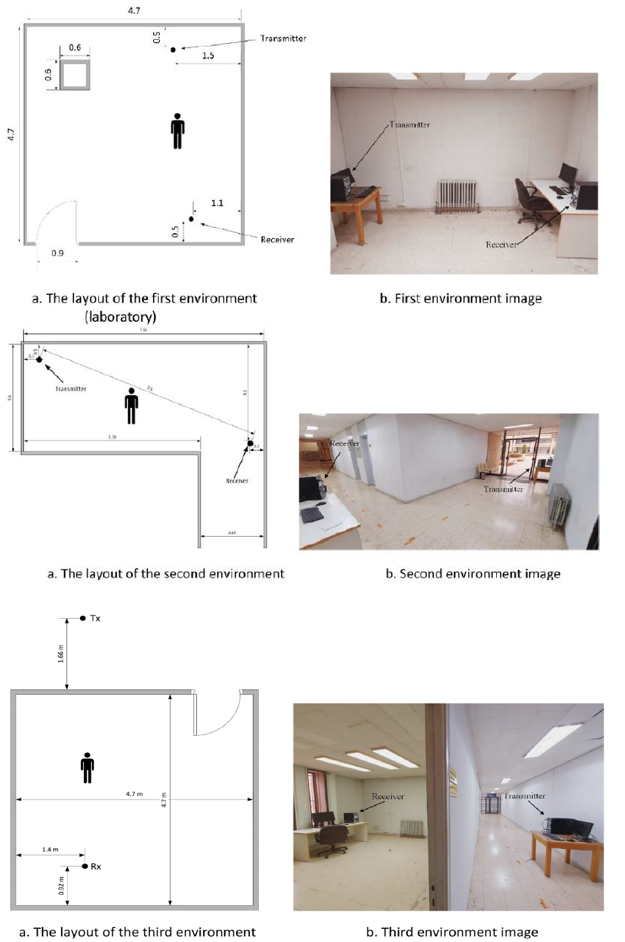
\includegraphics[scale=0.5]{images/Room Environment.png}}
\caption{Schematics of the Experiment Rooms}
\label{fig_room_schematics}
\end{figure}

\subsection{Data Preprocessing}
The CSI data provided by the Intel 5300 NIC is a set of complex numbers, which need to be processed by interpolating amplitude, phase and frequencies. Over that resultant interpolation, we can apply any denoising filter to smooth the wave forms. We have selected Discrete Wavelet Transform (DWT) filter for this case. Afterward, we need to select specific number of subcarriers ranging from 1 to 30 and select varying number of CSI data per batch to feed into our classifier. In between these preprocessing and classification steps, we can have an extra step to generate and extract specific features out of the filtered CSI data as amplitude, frequency, phase, etc.
Another step before feeding these data to the classifier would be to split it into 70\% training set \& 30\% test set.

\begin{figure}[htbp]
\centerline{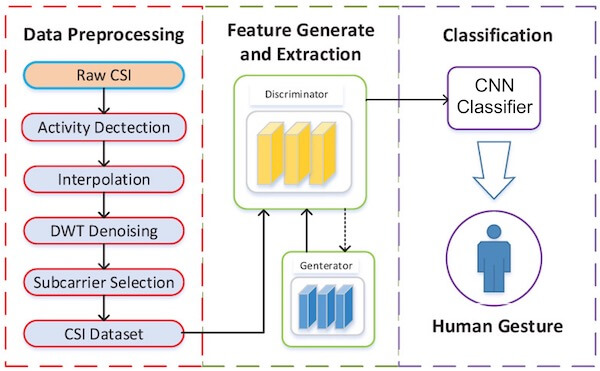
\includegraphics[scale=0.4]{images/steps_wifi_sensed_ml.jpg}}
\caption{Steps to Classify WiFi Sensed CSI data for Human Actions}
\label{fig_steps_wifi_sensing_ml}
\end{figure}


\subsection{Deep Learning Model}
Once the CSI data are denoised, we can make a machine learn from the dataset using any neural-network algorithm. We choose Convolutional Neural Network (CNN) to run over the dataset and classify each action among any of the ten predefined classes of human gestures. As shown in the steps the figure \ref{fig_train_steps}, we need to run multiple iterations of the model evaluation until a predefined number of epochs with the same dataset. The resultant model would be tested again by modifying any of the parameters of the model as well as of the dataset like number of subcarriers and CSI windows size. At a certain point of these optimization steps, we are most likely to have a model delivering high accuracy during evaluation of the model using our test dataset. At that point, we can finalize the model and complete our experiment.

\begin{figure}[htbp]
\centerline{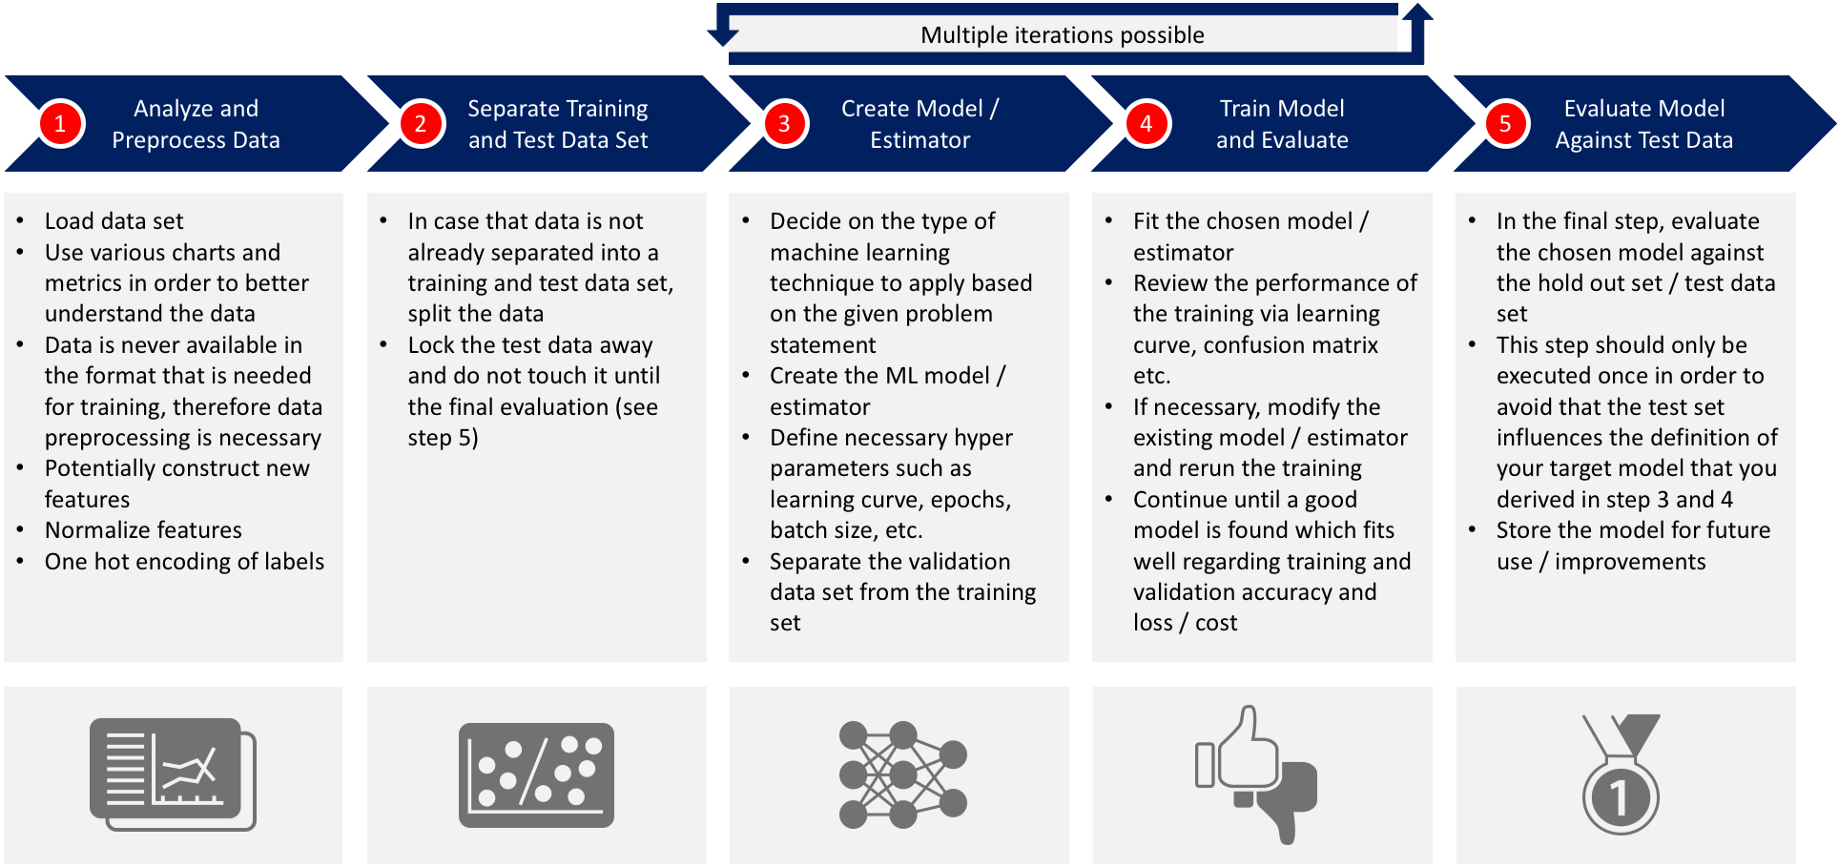
\includegraphics[scale=0.15]{images/train_steps.png}}
\caption{Data Preprocessing to ML Training \& Testing Steps \cite{img_har_categories} \cite{imu_lidar}}
\label{fig_train_steps}
\end{figure}

\section{Implementation Details}
We have designed the neural network with 5 layers in total, as illustrated in the Fig. \ref{fig_csi_cnn}.\\
Firstly, the CSI data are divided into chunks of 90 signals, each having 3*30=90 amplitudes as one per 90 subcarriers. So, one chunk has 90*90=8100 consecutive CSI data points converted to amplitudes, thereby, a square image is shaped for a chunk of CSI data. Moreover, each chunk is ensured to contain CSI of just one activity label, so that we can pass this square-shaped chunk into a convolution layer to be considered as a single image with a specific activity label and thereby learn using this image and also predict by the trained model.\\
In addition to these considerations, a significant part of this size is - as we have uniform 256Hz frequency for all the CSI data, each chunk having 90 signals actually mean (90/256) or 0.352 seconds of actions. So, a reasonable batch-size over these chunks can denote a specific duration of the data-collection process. For example, if we consider 256 as the batch-size, then the CSI data denotes a specific action being done over the duration, \\
$t = batch\_size\ \times\ image\_height \div frequency$ \\
$=(256 \times 90 \div 256)\ seconds$ \\
$= 256\ seconds$ \\
$= 4\ minutes\ and\ 16\ seconds.$\\

However, this understanding during the implementation phase is also found to be critical in learning with this set of CSI data, which is explained in the section \ref{section_results}.

As the Fig. \ref{fig_csi_cnn} shows, we have passed each of the such formed CSI image into a convlutional layer. The input map of this layer is always set to 1, as to expect one image at a time. We studied filters with size $3\times3$ and $5\times5$. We have experimented with the number of filters ranging from 5 to 180 for this layer, but conveniently found that lower number of filters actually works faster with pretty much good accuracy. The pooling layer always has the size of $2\times2$ and stride is always 1. We have not used any padding and used ReLU activation function for this implementation.\\
In the second convolution layer, we have used twice the number of filters in the first layer and all the other values, like - stride, pool-size \& padding, are kept the same. Then we needed to reshape the output of this layer into a one-dimensional format so that we can process this with the next dense layer with $12\times256$ number of outputs, which are then fed into another dense layer to generate 12 outputs each indicating the probability of one of the 12 activities. The highest probability is then considered as the predicted output. Upon having this result, the loss and the accuracy are calculated.\\
We have used TensorFlow library version 2.8.0 and Python 3.8 to implement this neural network. 

\begin{figure*}[htbp]
\centerline{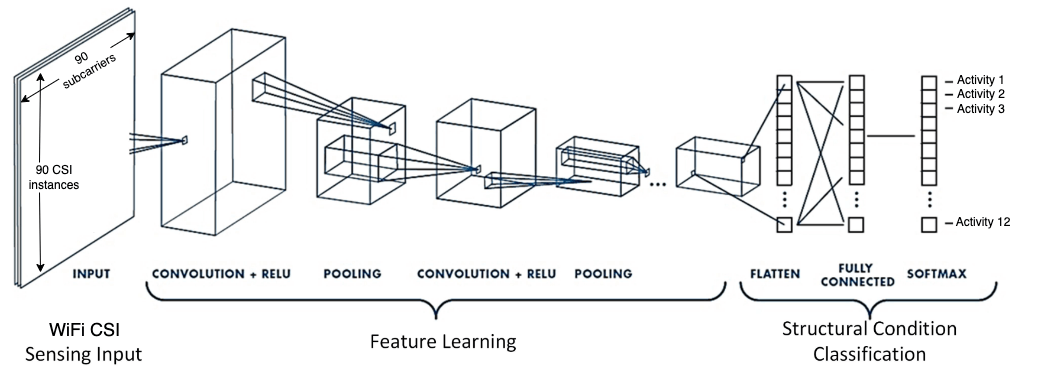
\includegraphics[scale=0.4]{images/csi_cnn.png}}
\caption{Depiction of the Designed CNN for the CSI data}
\label{fig_csi_cnn}
\end{figure*}


\section{Experimental Setup}
We have run our implementation for several epochs and several batches to find the optimal number of filters and batch-size, while we kept the image size ($90\times90$), pool-size, and number of layers constant. The experiments were run in the Tesla server at VCU HPC \cite{vcu_hpc}. The server has 2 Intel Xeon X5680 (3.33 GHz) processors with 24 cores, 96 GB RAM and 4 × NVIDIA Quadro P4000 (32GB) GPUs with 1792 CUDA cores.\\
Other than this instance, we have also run a few of the experiments in the VCU Maple server with 2 Intel Xeon E5-2690 (2.60GHz) processors with 56 cores in total and 378 GB RAM and 2 NVIDIA GeForce GTX 1080 Ti GPU with 3584 CUDA cores. All of the results are taken as average from these 2 instances. 

\section{Analysis of the Results}
\label{section_results}
We have varied the filter-size, number of filters, pool-size and the batch-size for our experiments. We have found out that only the batch-size has significant impact on the overall accuracy of our CNN implementation for this specific dataset. Furthermore, the lower batch-size always generates very low accuracy, i.e., below $30\%$, whereas the base accuracy for our 12 classes is $8.33\%$. For batch size of 256 and higher, we have achieved much satisfactory validation accuracy, as high as $73.3\%$.

The table \ref{table:result_epochs} shows the evolution of accuracy over all the epochs of our experiments. The table \ref{table:result_mean_high} shows that the higher batch-sizes yield better results for this dataset. We have achieved the highest accuracy as well as the highest average accuracy over all the epochs for a batch-size of 1536, which means that the best result is achieved when a single batch consisting of a specific duration of consecutive actions. This duration can be calculated as, \\
$t = batch\_size\ \times\ (image\_height \div frequency)$\\
$=(1536 \times 90 \div 256)\ seconds$\\
$= 540\ seconds$ \\
$= 9\ minutes.$\\


As the dataset was collected with a clocked set of actions and this batch size has no fraction of seconds, so we can relate this batch-size with the fact that a rounded set of actions is best suited to train with our implemented convolutional neural network, at least for this well-timed dataset.\\
The effect of batch size in our experiements can be well visualized in the Fig. \ref{fig_result_all}, where we can see that the line-chart for batch size of 1536 is almost always at the top of other line-charts for other batch sizes. The Fig. \ref{fig_result_mean} supports this claim by showing that the mean accuracy for batch size of 1536 is much higher than the other ones, where the other ones does not fluctuate that much and all are below the $40\%$ benchmark. The Fig. \ref{fig_result_highest} shows the highest accuracy of $73.3\%$ is achieved with the batch size of 1536, whereas its neighbouring batch sizes, i.e., 1024 and 2048 are not that much far from this peak and accuracies as $69.8\%$ and $68.2\%$ respectively.

It is worth mentioning that all of these metrics are collected over the average of multiple experiments with varying filter-size, pool-size and number of filters at each layer of the designed neural network. We have experimented filter-size of $3\times3$ and $5\times5$ with almost same average accuracy for all the batch-sizes. Similarly, the pool-size was varied for $2\times2$ and $4\times4$, along with number filters as 5, 9, 10, 15 \& 32. We got out-of-memory error even with the 32GB of GPU memory enabled server with number of filters larger than 32. But the other variables did not give any significant variation and so we have skipped these variables from our points of interest. 

Finally, it can be concluded that, a rounded set of actions per batch is well suited to train with our designed neural network. It is acceptable that there may be other latent hidden parameters which can be optimized to achieve even higher accuracy with our approach, like the varying the number \& type of layers. However, the accuracy can still be accepted as a fair achievement in reference to the studies of Alazrai et. al. \cite{csi_dataset_recent_refer1} which achieves $69.78\%$ accuracy with all these 12 actions of the same dataset and Alsaify et. al.\cite{csi_dataset_recent_refer2} which achieves $94\%$ accuracy with just 6 actions from this same dataset.


\begin{table}
% \begin{center}
     \begin{tabular}{| m{0.75cm} | m{1cm}| m{1cm} | m{1cm} | m{1cm} | m{1cm} |}
     \hline
        \multirow{2}{2em}{Epoch Number} & \multicolumn{5}{|c|}{Batch Size}\\ [1ex]
        \cline{2-6}
                     & 256 & 512 & 1024 & 1536 &  2048\\ [1ex]
        \hline\hline
                 5 	& 13.9 	& 15.1 	& 14.2 	& 14.8 & 10.8\\ [1ex]
         \hline
                 10	& 27.9	& 14.3	& 24.9	& 41.5 & 19.7\\ [1ex]
         \hline
                15	& 30.7	& 30.8	& 25.6	& 11.6 & 33.5\\ [1ex]
        \hline
                20	& 39.8	& 25	& 40.9	& 42.9 & 26\\ [1ex]
        \hline
                25	& 47.7	& 21.7	& 69.8	& 33.8 & 30.7\\ [1ex]
        \hline
                30	& 25.3	& 24.6	& 36.6	& 46.7 & 30.9\\ [1ex]
        \hline
                35	& 29.6	& 24.5	& 40.7	& 40.2 & 39.4\\ [1ex]
        \hline
                40	& 26.2	& 30.7	& 47.7	& 38.6 & 24.8\\ [1ex]
        \hline
                45	& 35.7	& 32.1	& 32.3	& 38.5 & 67.6\\ [1ex]
        \hline
                50	& 50.5	& 37.8	& 27.7	& 49.1 & 23\\ [1ex]
        \hline
                55	& 53.1	& 30.1	& 40.4	& 56.7 & 68.2\\ [1ex]
        \hline
                60	& 44.4	& 42.5	& 33	& 68.7 & 27.1\\ [1ex]
        \hline
                65	& 55.7	& 32.6	& 38	& 73.3 & 34\\ [1ex]
        \hline
                70	& 27.6	& 63.1	& 30.5	& 64.9 & 50.4\\ [1ex]
        \hline
                75	& 47.8	& 48.3	& 50.2	& 46.9 & 47\\ [1ex]
        \hline
                80	& 37.2	& 52.4	& 58.3	& 53.5 & 50.9\\ [1ex]
        \hline
                85	& 50.4	& 43.9	& 39.8	& 49.1 & 52.4\\ [1ex]
        \hline
                90	& 40.5	& 57.6	& 44.8	& 52.0 & 40.4\\ [1ex]
        \hline
                95	& 58.9	& 40.8	& 32.1	& 44.8 & 54.1\\ [1ex]
        \hline
                100	& 56.5	& 42.2	& 49.3	& 53.7 & 47.2\\ [1ex]
        % \hline\hline
        %         Mean & 39.97 & 35.505 & 38.84 & 46.065 & 38.905\\ [1ex]
        % \hline\hline
        %         Highest & 58.9 & 63.1 & 69.8 & 73.3 & 68.2\\ [1ex]
     \hline\hline
     \end{tabular}
 \caption{\label{table:result_epochs}Validation Accuracy of the designed CNN at several Epochs}
 \end{table}

\begin{table}
% \begin{center}
     \begin{tabular}{| m{0.75cm} | m{1cm}| m{1cm} | m{1cm} | m{1cm} | m{1cm} |}
     \hline
        \multirow{2}{3em}{Epoch Number} & \multicolumn{5}{|c|}{Batch size}\\ [1ex]
        \cline{2-6}
                     & 256 & 512 & 1024 & 1536 &  2048\\ [1ex]
        \hline\hline
                Mean & 39.97 & 35.505 & 38.84 & 46.065 & 38.905\\ [1ex]
        \hline
                Highest & 58.9 & 63.1 & 69.8 & 73.3 & 68.2\\ [1ex]
      \hline\hline
     \end{tabular}
\caption{\label{table:result_mean_high}Average \& Highest Accuracy Over 100 epochs}
\end{table}

\begin{figure}[htbp]
\centerline{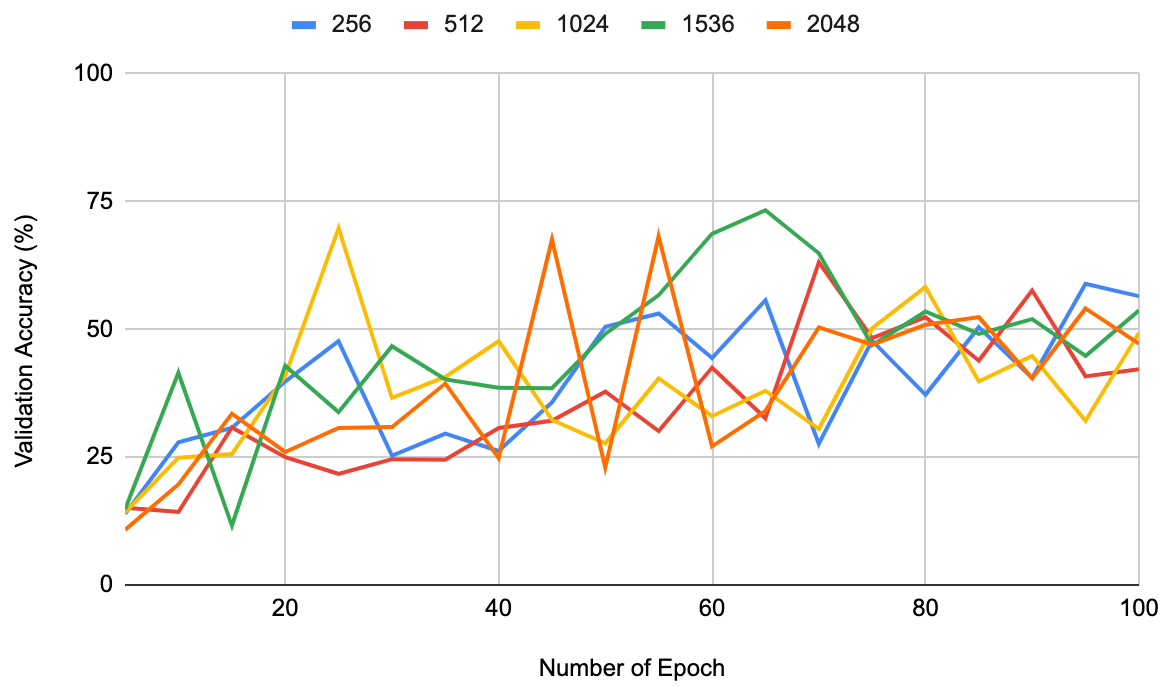
\includegraphics[scale=0.22]{images/bs_acc_all.png}}
\caption{Batch size vs validation-accuracy over all epochs}
\label{fig_result_all}
\end{figure}

\begin{figure}[htbp]
\centerline{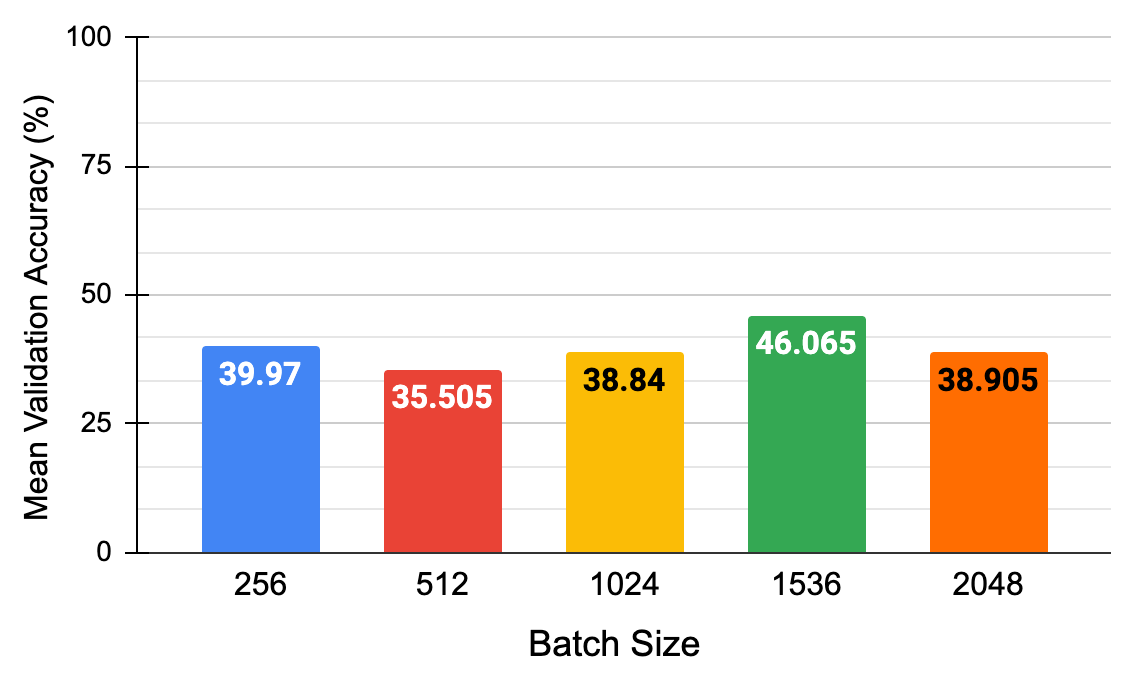
\includegraphics[scale=0.22]{images/bs_acc_mean.png}}
\caption{Batch size vs Mean validation-accuracy}
\label{fig_result_mean}
\end{figure}

\begin{figure}[htbp]
\centerline{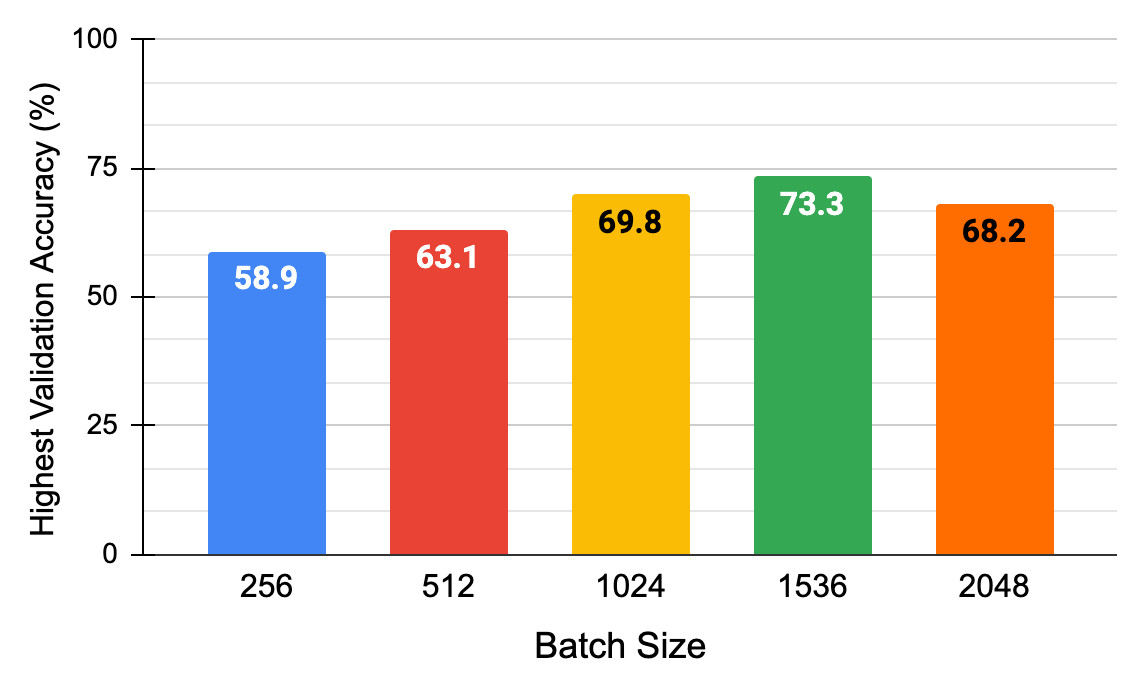
\includegraphics[scale=0.22]{images/bs_acc_highest.png}}
\caption{Batch size vs Highest Validation Accuracy}
\label{fig_result_highest}
\end{figure}


\section{Scopes of Future Studies}
For our future scopes of studies on this topic, we can certainly take the below par accuracy as the primary focus. We can vary the number of layers, as well as the concolution and dense types of layers with varying degree of combinations to find out which combination can work the best.

Along with these, we can also try with several activation functions instead of only ReLU activation function as done in this study. We have used softmax in the final layer, but there can be still a scope of improvement by using other functions at this layer. Other than these, we have studied with a very small number of variations of the filter size and the pool size, with which no significant difference is found. But these two can also be points of interest for some other combination of the parameters. 

Application of other denoising filters rather than the DWT filter and selection of specific subcarriers instead of selecting all of them as we have done in this study can also be some other non-ML scopes to study with our approach.

Using the same dataset, we can also try to classify the class-of-actions as shown in the table \ref{tabtable_subjects} and also the person doing the activities as different person has different approach to do a certain action and WiFi sensing approach is theoretically capable of collecting such subtle differences.

A certain other scope of future study is to try our designed neural network with other available datasets and thereby to test the robustness of our approach. 


\section{Conclusion}
%data format, cnn - novel, accuracy - almost acceptable in comparison to
We can come to a conclusion that our approach works slightly better than other similar studies with a novel application of CNN. There are a good amount of scopes to improve the accuracy of our approach, but it is certainly a good start with this comparatively newer dataset. The tested dataset is very well timed and so mostly dependent on the selection of batch size as found in our experiments. The other datasets may be more challenging for our approach, especially if that contains random and so practical human actions. For a comparatively newer paradigm of machine learning with WiFi sensing, this study can be considered as a contributing one and can be continued for many future studies.

%% \section*{Acknowledgment}
%% TODO write acknowledgment


\begin{thebibliography}{00}

\bibitem{har_jiang}Jiang W, Miao C, Ma F, Yao S, Wang Y, Yuan Y, Xue H, Song C, Ma X, Koutsonikolas D, Xu W. Towards environment independent device free human activity recognition. InProceedings of the 24th Annual International Conference on Mobile Computing and Networking 2018 Oct 15 (pp. 289-304).

\bibitem{har_csi}Palipana, Sameera, Piyush Agrawal, and Dirk Pesch. "Channel state information based human presence detection using non-linear techniques." Proceedings of the 3rd ACM International Conference on Systems for Energy-Efficient Built Environments. 2016.

\bibitem{intel_nic_device} https://dhalperi.github.io/linux-80211n-csitool/

\bibitem{a1}Zheng Yang et al. ''From rssi to csi: Indoor localization via channel response.'' \textit{ACM Comput. Surv.}, 46(2):25:1–25:32, December 2013.
\bibitem{a2} Z. Zhou et al. Towards omnidirectional passive human detection. In Proc. of INFOCOM, 2013.
\bibitem{a3} Jiang Xiao et al. Find: Fine-grained device-free motion detection. In Proc. of ICPADS, 2012.
\bibitem{dataset} Baha’ A. Alsaify, Mahmoud M. Almazari, Rami Alazrai, Mohammad I. Daoud,
A dataset for Wi-Fi-based human activity recognition in line-of-sight and non-line-of-sight indoor environments,
Data in Brief,
Volume 33,
2020,
106534,
ISSN 2352-3409,
https://doi.org/10.1016/j.dib.2020.106534.
\bibitem{imu_human} Semwal, V.B., Gaud, N., Lalwani, P. et al. Pattern identification of different human joints for different human walking styles using inertial measurement unit (IMU) sensor. Artif Intell Rev 55, 1149–1169 (2022). https://doi.org/10.1007/s10462-021-09979-x

\bibitem{pyroelectric_human1} Q. Hao, D. J. Brady, B. D. Guenther, J. B. Burchett, M. Shankar and S. Feller, "Human Tracking With Wireless Distributed Pyroelectric Sensors," in IEEE Sensors Journal, vol. 6, no. 6, pp. 1683-1696, Dec. 2006, doi: 10.1109/JSEN.2006.884562.

\bibitem{pyroelectric_human2} Q. Hao, F. Hu and Y. Xiao, "Multiple Human Tracking and Identification With Wireless Distributed Pyroelectric Sensor Systems," in IEEE Systems Journal, vol. 3, no. 4, pp. 428-439, Dec. 2009, doi: 10.1109/JSYST.2009.2035734.
\bibitem{img_har_categories} https://iesedmonton.org/news/2018-5-22/what-are-pir-sensors-and-why-do-i-need-them, https://www.wired.com/2010/11/tonights-release-xbox-kinect-how-does-it-work/, https://www.sourcesecurity.com/tags/thermal-imaging.html
\bibitem{mmWave_rf_vs_kinect_radar_img} Sizhe An and Umit Y. Ogras. 2021. MARS: mmWave-based Assistive Rehabilitation System for Smart Healthcare. ACM Trans. Embed. Comput. Syst. 20, 5s, Article 72 (October 2021), 22 pages. DOI:https://doi.org/10.1145/3477003
\bibitem{math_dervd_hand_pos_sensor} R. Abbasi-Kesbi and A. Nikfarjam, "A Miniature Sensor System for Precise Hand Position Monitoring," in IEEE Sensors Journal, vol. 18, no. 6, pp. 2577-2584, 15 March15, 2018, doi: 10.1109/JSEN.2018.2795751.
\bibitem{wear_handglove} X. Chen et al., "A Wearable Hand Rehabilitation System With Soft Gloves," in IEEE Transactions on Industrial Informatics, vol. 17, no. 2, pp. 943-952, Feb. 2021, doi: 10.1109/TII.2020.3010369.
\bibitem{joints_imu}Ana Pereira, Vânia Guimarães, and Inês Sousa. 2017. Joint angles tracking for rehabilitation at home using inertial sensors: a feasibility study. In <i>Proceedings of the 11th EAI International Conference on Pervasive Computing Technologies for Healthcare</i> (<i>PervasiveHealth '17</i>). Association for Computing Machinery, New York, NY, USA, 146–154. DOI:https://doi.org/10.1145/3154862.3154888

\bibitem{rokoko_link} https://www.rokoko.com/
\bibitem{ultraleap} https://www.ultraleap.com/

\bibitem{imu_lidar} Patil, Ashok Kumar \& Balasubramanyam, Adithya \& Ryu, Jae \& B N, Pavan Kumar \& Chakravarthi, Bharatesh \& Chai, Young-Ho. (2020). Fusion of Multiple Lidars and Inertial Sensors for the Real-Time Pose Tracking of Human Motion. Sensors (Basel, Switzerland). 20. 10.3390/s20185342. 


\bibitem{dalal} Dalal N., Triggs B., Schmid C. (2006) Human Detection Using Oriented Histograms of Flow and Appearance. In: Leonardis A., Bischof H., Pinz A. (eds) Computer Vision – ECCV 2006. ECCV 2006. Lecture Notes in Computer Science, vol 3952. Springer, Berlin, Heidelberg. https://doi.org/10.1007/11744047\_33

\bibitem{yun_pir} Yun, J.; Lee, S.-S. Human Movement Detection and Identification Using Pyroelectric Infrared Sensors. Sensors 2014, 14, 8057-8081. https://doi.org/10.3390/s140508057

\bibitem{young_impulse_radar} Young-Jin Park, Hui-Sup Cho (2020) A Method for Detecting Human Presence and Movement Using Impulse Radar, Division of Electronics \& Information System, DGIST, Daegu, 42988, South Korea

\bibitem{jeong_thermal}Y. Jeong, K. Yoon and K. Joung, "Probabilistic method to determine human subjects for low-resolution thermal imaging sensor," 2014 IEEE Sensors Applications Symposium (SAS), 2014, pp. 97-102, doi: 10.1109/SAS.2014.6798925.

\bibitem{semwal}Semwal, V.B., Gaud, N., Lalwani, P. et al. Pattern identification of different human joints for different human walking styles using inertial measurement unit (IMU) sensor. Artif Intell Rev 55, 1149–1169 (2022). https://doi.org/10.1007/s10462-021-09979-x

\bibitem{deman}C. Wu, Z. Yang, Z. Zhou, X. Liu, Y. Liu and J. Cao, "Non-Invasive Detection of Moving and Stationary Human With WiFi," in IEEE Journal on Selected Areas in Communications, vol. 33, no. 11, pp. 2329-2342, Nov. 2015, doi: 10.1109/JSAC.2015.2430294.

\bibitem{domenico} S. Di Domenico, M. De Sanctis, E. Cianca and M. Ruggieri, "WiFi-based through-the-wall presence detection of stationary and moving humans analyzing the doppler spectrum," in IEEE Aerospace and Electronic Systems Magazine, vol. 33, no. 5-6, pp. 14-19, May-June 2018, doi: 10.1109/MAES.2018.170124.

\bibitem{hernandez_one_sided_wall}S. M. Hernandez and E. Bulut, "Adversarial Occupancy Monitoring using One-Sided Through-Wall WiFi Sensing," ICC 2021 - IEEE International Conference on Communications, 2021, pp. 1-6, doi: 10.1109/ICC42927.2021.9500267.
\bibitem{hernandez_wifederate}S. M. Hernandez and E. Bulut, "WiFederated: Scalable WiFi Sensing using Edge Based Federated Learning," in IEEE Internet of Things Journal, doi: 10.1109/JIOT.2021.3137793.

\bibitem{csi_human}Sameera Palipana, Piyush Agrawal, and Dirk Pesch. 2016. Channel State Information Based Human Presence Detection using Non-linear Techniques. In <i>Proceedings of the 3rd ACM International Conference on Systems for Energy-Efficient Built Environments</i> (<i>BuildSys '16</i>). Association for Computing Machinery, New York, NY, USA, 177–186. DOI:https://doi.org/10.1145/2993422.2993579

\bibitem{liu_breathing} Y. Liu, H. Liu and F. Gao, "Channel State Information-based Device-Free stationary Human Detection with estimating respiratory frequency," 2019 IEEE 4th Advanced Information Technology, Electronic and Automation Control Conference (IAEAC), 2019, pp. 1111-1117, doi: 10.1109/IAEAC47372.2019.8997815.

\bibitem{vcu_hpc}https://wiki.vcu.edu/display/EGRITHELP/HPC+-+EGR+-+Departmental+HPC+Resources

\bibitem{csi_dataset_recent_refer1}R. Alazrai, A. Awad, B. A. Alsaify and M. I. Daoud, "A Wi-Fi-based Approach for Recognizing Human-Human Interactions," 2021 12th International Conference on Information and Communication Systems (ICICS), 2021, pp. 251-256, doi: 10.1109/ICICS52457.2021.9464570.

\bibitem{csi_dataset_recent_refer2} B. A. Alsaify, M. M. Almazari, R. Alazrai and M. I. Daoud, "Exploiting Wi-Fi Signals for Human Activity Recognition," 2021 12th International Conference on Information and Communication Systems (ICICS), 2021, pp. 245-250, doi: 10.1109/ICICS52457.2021.9464613.

\end{thebibliography}

\end{document}
© 2022 Overleaf English|Privacy and TermsSecurityContact UsAboutBlogOverleaf on TwitterOverleaf on FacebookOverleaf on LinkedIn